\Chapter{Design}
Now, after having discussed the necessary concepts and ideas required to fully understand the mathematical model of the interpreter we can finally start inspecting its design requirements, what aspects must be taken into consideration, the language of choice, compatibility related questions etc. Regarding the task of interpretation, these types of programs conform to a specific pipeline that largely determines their architecture. With that said there is still leeway for flexibility and that allows us to adept and choose adequate data structures along with various techniques and algorithms for controlling data flow.

\Section{Requirements and Technical Considerations}
Due to past research around fuzzy logic and its application in behavior control the need for having an adequate language along with a library or interpreter to make calculations easier also arose. For avoiding ambiguity, in the following discussions the terms library, program and interpreter are used interchangeably and should be treated as referring to the same concept, namely the FBDL interpreter. The entire operation of the program is based on the preceding works and research in fuzzy behavior control and behavior-based systems \cite{pillerkovacs2019}.

Many of the applied examples were produced in the MATLAB language, therefore facilitating the need for  developing a framework capable of operation in that environment. The similarity between the MATLAB and Octave programming languages presented a great opportunity; implementing the interpreter in such a way as to conform to both languages would make it more accessible and allow for wider usage. Therefore the decision was made to produce a program that uses in its operation only minimal parts that are found in both languages, thus making it compatible and interoperable.

To further elaborate, the usage of language specific components and features should be kept at a minimum or avoided altogether if possible, for example the definition of classes or application of several built in functions, function definitions, unit tests etc. are such areas where the two target languages tend to differ quite majorly. It also does not help that at each iteration and new versions these differences grow ever larger since new features are added and perhaps old ones modified or removed, hence implementation with only basic and fundamental features of each language should be prioritized to the utmost extent.


\Section{Structure of The Interpreter}
The difference in function definitions, the most noticeable one being that in MATLAB scripts cannot contain any local function definitions before version R2016b, and also other incompatibilities related to the syntax of this operation are the main reason that the program is organized in a way so that every function definition occupies its own $.m$ file. 

Since the interpreter is not a standalone program, rather a library, its entry point is a function that gets called from the user of this library. From there it goes through each stage of interpreting the input; it is comprised of 3 major parts and a lot of smaller, auxiliary functions that help in completing the task, along with making the program code more readable and modular as depicted on figure \ref{fig:tree}.

\begin{figure}[!h]
	\centering
	\begin{forest}
	  for tree={
	    font=\ttfamily,
	    grow'=0,
	    child anchor=west,
	    parent anchor=south,
	    anchor=west,
	    calign=first,
	    edge path={
	      \noexpand\path [draw, \forestoption{edge}]
	      (!u.south west) +(7.5pt,0) |- node[fill,inner sep=1.25pt] {} (.child anchor)\forestoption{edge label};
	    },
	    before typesetting nodes={
	      if n=1
	        {insert before={[,phantom]}}
	        {}
	    },
	    fit=band,
	    before computing xy={l=15pt},
	  }
	[Interpreter
		[main.m \textit{(Entry point)}]
		[lexer
			[utils
				[\textit{Utility programs}]
			]
		    	[getNextToken.m]
		    	[\textit{Lexical analyzer functions}]
		  ]
	 	 [parser
	    		[parer.m]
	    		[\textit{Parsing functions}]
			[\textit{Semantic checkers}]
	  	]
		[engine
	    		[\textit{Integrity checkers}]
	    		[\textit{Calculating functions}]
	  	]
	]
	\end{forest}
	\caption{Interpreter file hierarchy}
	\label{fig:tree}
\end{figure}

The program's entry point is a callable function that takes either a string or a file path as input and returns the solution vectors resulting from the fuzzy calculations. In both cases the content supplied must be a valid piece code written in FBDL. 

\begin{octave}
function engine = simulator(input, type)
  retval = 0;
  addpath("lexer");
  addpath("lexer/utils");
  addpath("parser");
  addpath("engine");

  content =  "";
  if strcmp(type, "f")
    content = fileread(input);
  elseif strcmp(type, "s")
    content = input;
  else
    print_usage();
  end

  behavior = parser(content);
  engine = createEngine(behavior);
  engine = init(engine);
end
\end{octave}

Functions that facilitate the usage of the program must first be ``included'' with path definitions treating the above entry point as root, since they are stored in their separate files. Supplying the function with either type of valid input will initiate its operation, anything other than that will result in an error and the user will be provided a message on basic usage.

The function $parser()$ being called first might be a bit counter intuitive, but the lexer and parser operate simultaneously, not in a procedural manner, where the output of the lexer is the input to the parser. Of course doing it that way is also possible, returning a vector of tokens and then parsing that, however it is not just less efficient, but at the same time takes away the ability to report errors with correct positional messages, since that information is carried by the lexer and not the tokens.

\begin{figure}[!h]
	\centering
	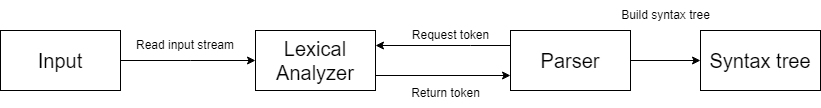
\includegraphics[width=1\textwidth]{images/parserOperation}
	\caption{Pipeline up to the parser}
	\label{fig:parserOp}
\end{figure}

As seen on figure \ref{fig:parserOp}, the parser continuously requests tokens from the lexer and at the same time it builds the syntax tree for the entire program, after which this completed structure is passed to the engine for calculations.

\Section{Data Structures}
Regarding the data structures used in the program, the most compatible with both languages were found to be the \textit{struct} and \textit{cell}, hence all complex objects are stored in such a manner. For clarity,  the \textit{cell} data type is not used as frequently, but in some parts it is more appropriate than other solutions. The most important of these objects is the \textit{lexer}, but others include \textit{token} and the \textit{syntax tree} along with other minor internal data structures that store and manage the information read during or after lexical analysis.

\SubSection{Lexer}
This structure holds the input and several key information about the position of the cursor currently analyzing the text. Due to organizing every function into its own file the lexer can only be either a global structure that gets modified by any given function or it is created locally in the top most function in terms of calling hierarchy and is passed around by every other function that needs either access to the input stream or the metadata stored in it. A separate function for creating a lexer is provided in foresight to unit testing, so as to avoid having to create it in every single test case.

\begin{octave}
function lexer = createLexer(content)
  keywords = {
    "universe", "rulebase", "end", "description", "rule",...
    "when", "and", "is", "init",  "use"
  };

  lexer = struct(
    "content", content,
    "content_len", length(content),
    "cursor", 1,
    "line", 1,
    "beginning_of_line", 1,
    "token_begins", 1
  );

  lexer.keywords = keywords;
end
\end{octave}

The input stream, or as \textit{content} in the lexer structure, is processed by one character at a time and the \textit{cursor} represents how many characters we have read so far, in other words our current position withing the supplied text. Lines are incremented with each encounter of a \textbackslash\textit{n (newline)} character. The staring position of the given token is also stored to allow for copying the value and report error messages, indicating the position of the incorrect token.

The more complex structures seen on figures \ref{fig:lexerUML}, \ref{fig:parserUML} and \ref{fig:engineUML} are defined as composites, where the rectangles with rounded corners indicate some sort of data, either primitive or a structure, and ellipses denote some ``methods'' these structures access. Though these figures resemble UML diagrams it is important to note that the structures presented are not classes; this is simply a logical view to better understand the overall building blocks of the interpreter.

\pagebreak

\begin{figure}
\centering
	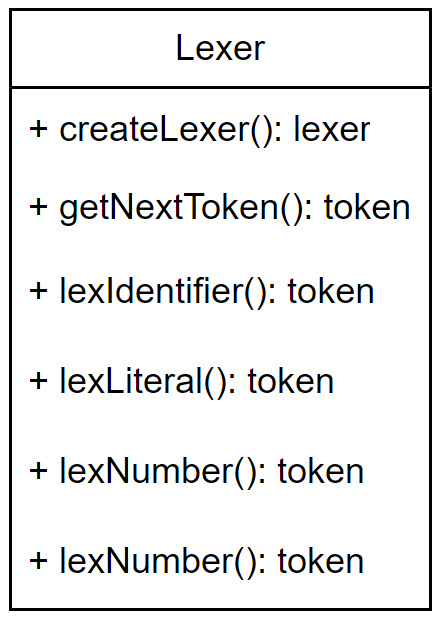
\includegraphics[width=0.4\textwidth]{images/lexerUML}
	\caption{Lexer Structure}
	\label{fig:lexerUML}
\end{figure}

\begin{figure}[!h]
\centering
\begin{subfigure}{.5\textwidth}
	\centering
	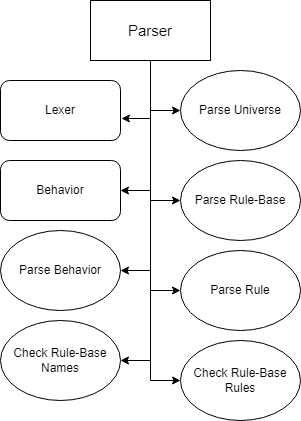
\includegraphics[width=0.8\textwidth]{images/parserUML}
	\caption{Parser}
	\label{fig:parserUML}
\end{subfigure}%
\begin{subfigure}{.5\textwidth}
	\centering
	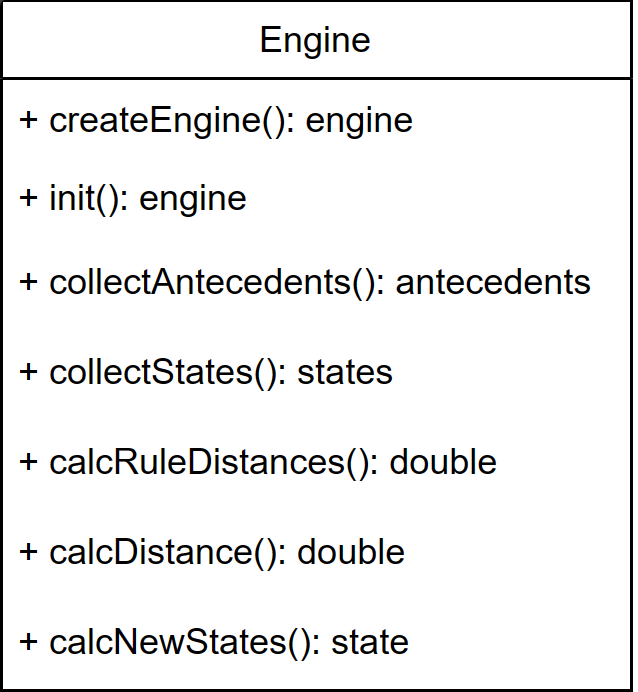
\includegraphics[width=0.8\textwidth]{images/engineUML}
	\caption{Engine}
	\label{fig:engineUML}
\end{subfigure}
\caption{Parser and Engine Structures}
\label{fig:paserengine}
\end{figure}

\SubSection{Token}
Defined as having the fields: type and value, where the former can be any of the valid token types described by the grammar rules of the FBDL and the latter takes on the actual value read from the input stream. Below are the types accepted and the possible values a token may take:

\begin{itemize}
	\item \texttt{keyword}: \textit{universe, rulebase, init, end, description, rule, when, and, is, use},
	\item \texttt{string}: \textit{Any character sequence between two '' (double quote) symbols},
	\item \texttt{number}: \textit{Any number, be it decimal or whole with . (dot) for separator in case of the former},
	\item \texttt{identifier}: \textbf{RESERVED} \textit{Any ASCII alphanumeric sequence starting with either a letter or \_ (underscore)},
	\item \texttt{terminal}: \textbf{RESERVED} \textit{Special symbols such as (), ::, \{\}, []}.
\end{itemize}

\textit{Please note that tokens designated as \textbf{reserved} are either already in the program code, but not actively used or there are room for them should the need arise for future extension.}

Tokens are ``produced'' or emitted by the \textit{emitToken}  function that constructs a token structure with the correct type and value.

\begin{octave}
function token = emitToken (type, value)
  token = struct(
    "type", type,
    "value", value);
end
\end{octave}

\SubSection{Syntax Tree}
During the process of parsing, every element of the language must be stored for later processing and calculations by the engine. The final structure resembles a tree, hence the name, and mimics the grammar of the language; it is a composite of all the objects defined within the code. Parts that may appear multiple times or none at all are stored in structure/cell fields with their names in order to achieve access similar to that of a hash table; in another case, where the given objects must be iterable they are stored as lists and all these list elements contain the name of the object along with other properties, such as values or further embedded structures. Both the hash table and the list provide sufficient storage and access capabilities, however each have their drawbacks regarding the method by which elements can be reached. The information and data used by the engine for calculations does most of the access and therefore the nature of these structures must be carefully considered beforehand to facilitate ease of use and smooth operations.

\begin{figure}[!h]
	\centering
	\begin{forest}
		 [behavior
		 	[universe
				[symbol
					[string]
					[number]
					[number]
				]
			]
		 	[rulebase
				[rules
					[string]
					[predicates
						[string]
						[string]
					]
				]
			]
		 ]
	\end{forest}
	\caption{Syntax tree}
\end{figure}

The representation is only logical and not entirely accurate as it would take too much space to represent it in its whole from, but nonetheless it offers another clear depiction of the grammar besides BNF, EBNF and railroad diagrams.

